\chapter{Személyfelismerés algoritmusának kialakítása mobil roboton}
\label{sec:algo}
A fejezetben ismertetem az általam tervezett algoritmus működését, a programozott megoldás felett egy absztrakciós szinttel. Leírom a felhasznált eszközöket, fő könyvtárakat, illetve modulokat, s azok kiválasztásának indokait. Kitérek az algoritmus működésének fontos lépéseire, a megvalósításukat a következő (\refstruc{sec:inros}ben) írom le.

\section{face-recogniton modul}
\label{sec:facerec}
Arcok felismerésére és manipulálására készült Python könyvtár \cite{artc31}. Választásom fő indoka, hogy megfelelően pontos: 99,38\%-os pontosságot ért el a „Faces in the Wild benchmark”-on\footnote{Labeled Faces in the Wild: \url{http://vis-www.cs.umass.edu/lfw/}} és használata egyszerű. Lehetővé teszi az arcok felismerését, a különböző arcvonások (mint például a szemek, az orr és az ajkak) megjelölését, valamint a különböző arcok összehasonlítását. A „face-recognition" könnyen használható, és segítségével egyszerűen lehetővé válik az arcok felismerése képeken és videókon. Egyszerűség alatt azt értem, hogy az elvárt funkciók, arcok észlelése egy képen, arcok összehasonlítása és egyezésük megállapítása, mind elvégezhetőek egy-egy függvényben akár parancssorban is. A Dlib legmodernebb arcfelmerésével készült, mély tanulással („deep learning"-el) épült \cite{artc31}.

Modulban megírt függvényekkel a felhasználó számára egyszerűen lehet elvégezni az arcfelismerést. A \verb|.load_image_file(„your_file.jpg")| függvényével a megadott képet beolvassa és tárolja egy változóban. Az arcokról úgynevezett „enkódolást" (encoding) hoz létre, ez az emberi arcok algoritmus által használt reprezentációja. A dolgozat további részében „enkódolás"-ként hivatkozok rá. Az „enkódolást" a modul \verb|.face_encodings(„image")| függvénye hozza létre. Egy listát ad vissza az arcok „enkódolásairól", mely annyi dimenziós, ahány embert észlelt a képen(„image"). Lehetőség van kép megadására fájl elérési útvonalával vagy az előző függvénnyel beolvasott változóval. Az arcok összehasonlítására, egyezésük megállapítására a \verb|.compare_faces(known_encodings, unknown_encoding)| függvény használható. Az „unknown\textunderscore encoding" argumentumban azt az „enkódolást" kell megadni amit össze szeretnénk hasonlítani a „known\textunderscore encodings" argumentumban megadottakéval (itt megadhatunk listát vagy egyetlen egy „enkódolást" is). A függvény kimenete egy „boolean" lista, amely a „known\textunderscore encodings" argumentumban megadott arcokkal való egyezést adja meg rendre (egy „enkódolás" megadása esetén egy elemű lista a kimenet).


\subsection{Dlib}
A Dlib\cite{dlib} egy nyílt forráskódú könyvtár, amely mesterséges intelligencia és számítógépes látás használatát igénylő feladatok megoldására használható különös tekintettel a számítógépes látás feladatokra, mint például a arc- és arcvonások felismerése. Képek és videók számítógépes elemzésére, valamint a gépi tanulás alapú megközelítések implementálására használható. A Dlib könyvtár C++ nyelven íródott. A Dlib-et széles körben használják a kutatók és fejlesztők intelligens rendszerek és alkalmazások fejlesztéséhez\cite{artc30}.

\section{Algoritmus feladatai}
%forrás: https://towardsdatascience.com/how-to-build-a-face-detection-and-recognition-system-f5c2cdfbeb8c
A projekt elején kettő felhasználási célt határoztunk meg, amik közül az egyik elérése jelentette az eredményességet. Az egyik felhasználás mód, hogy előre megadott embereket ismerjen fel az algoritmus, a másik, hogy képes legyen új emberek megjegyzésére. Végső soron mindkettő feladat ellátására képes a megalkotott csomag.

Egy általános arcfelismerő rendszer működéséhez három lépést kell végrehajtani. Először is észlelnie kell az arcokat a videókamera képén. Ezután optimális esetben azonnal fel kell ismernie ezt az arcot. Végül meg kell tennie a szükséges további lépéseket, ami ebben az esetben, hogy egy meghatározott kimeneten megjelenítse, milyen arcokat lát hozzájuk tartozó névvel \cite{artc32}.

 \clearpage

\section{Folyamat lépései}
Az arcfelismerő folyamat nulladik lépése, hogy elérjük a valós képet amit a robot lát.
Első lépés a kép elemzése, és a rajta található összes arc megkeresése. Feltétel, hogy észlelni tudjon arcokat különböző környezeti tényezők, például eltérő megvilágítás mellett, és lehetőség szerint az arc orientációja se akadályozza a keresést.
Második lépés, hogy képes legyen az arcokról egyedi tulajdonságaik alapján különböző emberek megkülönböztetésére alkalmas kimenetet generálni, például mekkora a szem, milyen hosszú az arc stb.
A harmadik lépés, hogy az arcra kapott egyedi adatokat hasonlítsa össze az eddig ismert arcokkal és határozza meg a legközelebbi egyezést, a legjobban hasonlító arcot és adja vissza az ehhez társított nevet.

\subsection{1. lépés: a kép feldolgozása}
Miután rögzítettük a kamera képét a következő szükséges lépés a feldolgozás. Ez alatt két lépést különíthetünk el: az arcok észlelése és felismerése. Az észlelés amikor az arcokat elkülönítjük a háttértől, gyakorlati egyszerűséggel fogalmazva az arcok és minden ami nem arc szétválasztása. A felismerés az ez utáni lépés, amikor az arcok között teszünk különbséget.

\subsection{2. lépés: az arcok észlelése}
Az arcok észlelése a 2000-es évek elején vált sokak számára elérhetővé, amikor Paul Viola és Michael Jones létrehoztak egy keretrendszert \cite{artc33} objektumok felismerésére.

Ezzel a keretrendszerrel annyira gyorssá vált az arcok detektálása, hogy már az alsó árkategóriás kamerák is képesek lettek rá. Ma azonban sokkal megbízhatóbb megoldások léteznek. Egy 2005-ben kifejlesztett módszert alkalmazó Python könyvtárat használok, a módszer neve: „Histogram of Oriented Gradients” - vagy röviden csak HOG \cite{artc34}.

\subsubsection{HOG működése}
Az algoritmus működése röviden: feldolgozandó adatmennyiség csökkentésére fekete-fehérré alakítja a HOG a képet, mivel plusz adat a színekről nem szükséges arcok észleléséhez. Ezután a képet felosztja egy rácsra, minden elemét egyesével vizsgálja. Minden egyes elemi rács négyzet esetében megnézi a közvetlenül mellette levő elemeket. Összehasonlítja mennyivel sötétebb az őt körülvevő képpontoktól, ebből gradiens vektort számol, ami megmutatja a kép melyik irányban sötétedik. Ezt a folyamatot a kép minden egyes képpontjával megismétli. Rács minden elemében vissza ad egy gradiens vektort.
Ahhoz, hogy arcokat észleljünk ezen a HOG-képen, csak meg kell találnunk a képünknek azt a részét (\refstruc{fig:hog}), amely a leginkább hasonlít arcokról készített ismert HOG-mintához \cite{artc_gold}\cite{artc35}.
\begin{figure}[!ht]
    \centering
    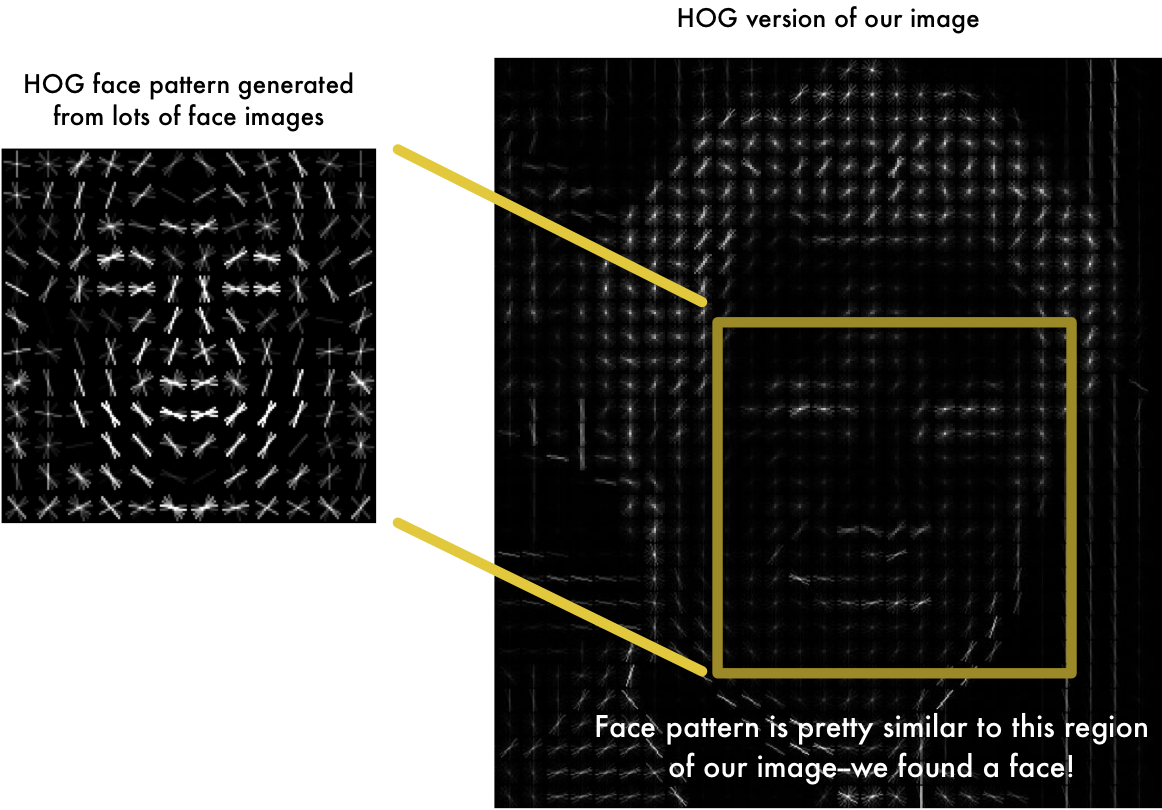
\includegraphics[width=100mm, keepaspectratio]{03_images/hog.png}
    \caption{HOG algoritmust demonstráló ábra \cite{artc_gold}.}
    \label{fig:hog}
\end{figure}

\subsubsection{Arcok orientációja}
Mivel egy valós környezetben az emberek nem mindig néznek a kamerába, így az arcukat különböző orientációkban, elfordulásokban rögzíti a kamera. Ezt figyelembevéve a „face-recognition” Python modul az arcokat transzformálja a feldolgozása során. Oly módon, hogy a szemek és az ajkak mindig ugyanazon helyen legyenek a képen. Ez megkönnyíti az arcok összehasonlítását.
Az arcok összehasonlításához a „face landmark estimation” algoritmust használja. Sokféle módja van két arc összehasonlításának ennek, de a modul a Vahid Kazemi és Joseph Sullivan által 2014-ben kifejlesztett megközelítést \cite{artc36} alkalmazza.
Az alapötlet, hogy definiálunk 68 specifikus pontot, ami minden arcon megtalálható. A pontokat a jellegzetes arcvonások mentén határozták meg, mint az áll, szemöldök, orr, ajkak és az arc körvonala, ahogyan a mellékelt \refstruc{fig:arcpontok} is szemlélteti.
\begin{figure}[!ht]
    \centering
    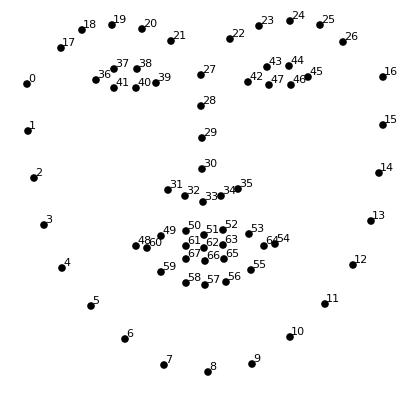
\includegraphics[width=75mm, keepaspectratio]{03_images/arcpontok.png}
    \caption{Arcot leíró jellegzetes pontok \cite{artc_gold}.}
    \label{fig:arcpontok}
\end{figure}

\subsection{3. lépés: arcok felismerése}
A felismerés lényege, hogy az emberi arcot leírjuk egy csak az egyénre jellemző módon. Kitétel, hogy az adattípus és formátuma összehasonlítható legyen az arcok között. A cél, hogy ugyanazt az arcot látva ez az adat megegyezzen, különböző arcok esetében pedig eltérőt kapjunk. Az emberek viselkedéséből kiindulva egy választás lehet a szem- vagy hajszín, arc formája, de ezek a paraméterek nem igazán értelmezhetőek egy számítógép számára, amely a kép egyes pixeleit vizsgálja. A kutatók rájöttek, hogy a legpontosabb megközelítés az, ha „hagyják”, hogy a számítógép maga találja ki az arcok összehasonlítását képező paramétereket és összegyűjtse ezeket az adatokat. Erre használt módszer a mély tanulás (deep learning), mely segítségével meghatározható, az arc mely részei fontosak a méréshez. A megoldás egy konvolúciós háló betanítása, amely minden egyes archoz meghatározott számú összehasonlítási pontot generál.

A korábban bemutatott Python-os „face-recognition” modul esetében, aminek Dlib az alapja egy 128 dimenziós vektort állít elő, ami részletesen leírja az arcvonásokat, az arc ismertető jegyeit. Ez a vektor alapján válik kvantálttá, gépi módon összehasonlíthatóvá az arc. A betanítás folyamat röviden leírva: gyakorló képeket biztosítunk a konvolúciós háló számára, melyekről megadjuk, hogy ki található rajtuk. Elvárjuk, hogy olyan 128 elemű vektort készítsen a képekről, melyek euklidészi térben értelmezve közel esnek egymáshoz (távolságuk minimalizálására törekszik), ha két azonos ember arcáról készültek. Távol esnek egymástól a vektorok, ha két különböző ember arcáról képet vizsgál. Megfelelő mennyiségű gyakorló képet biztosítva mély tanulás a háló paraméterei úgy módosulnak, hogy az előző két kitételt minél pontosabban hajtsa végre \cite{artc_gold}. Ezt a betínítást a „face-recognition” modul megalkotója már elvégezte, a \refstruc{sec:facerec}ban leírt pontosságot elérve.

\clearpage %Page break
\section{Hardveres tervezési szempontok}
\label{sec:sec-cam}
Mivel a Biscee robot már fel van szerelve az erre a célra megfelelő hardverrel, kettő BASLER acA1300-60gc kamerával (\refstruc{fig:cam}), így ez a feltétel már teljesült. Következő lépésként a kamera képéhez hozzá kell férni. A roboton futó ROS keretrendszer segítségével, melyet a \az+\refstruc{sec:inros}ben mutatok be, ez könnyen a megvalósítható. A ROS hasznos eszközöket biztosít a külső eszközök elérésére. A keretrendszeren belüli feldolgozáshoz egyértelmű választás volt az OpenCV Python nyelvre implementált modulja. A cél, hogy a feldolgozás valós időben dolgozzon, mert akkor ítélhető hasznosnak az információ, ha rögtön tudjuk kik vannak a robot látóterében. Emiatt fontos annak a csatorna sebességének az optimalizálása, amin keresztül eljut a kamerától az arcfelismerő kódban feldolgozhatóságig a kép. Szempontok, amiket tervezésnél nem lehet megkerülni: a gyorsaság, a minőség és a hardveres lehetőségek, azaz erőforrások használata.

\begin{figure}[!ht]
    \centering
    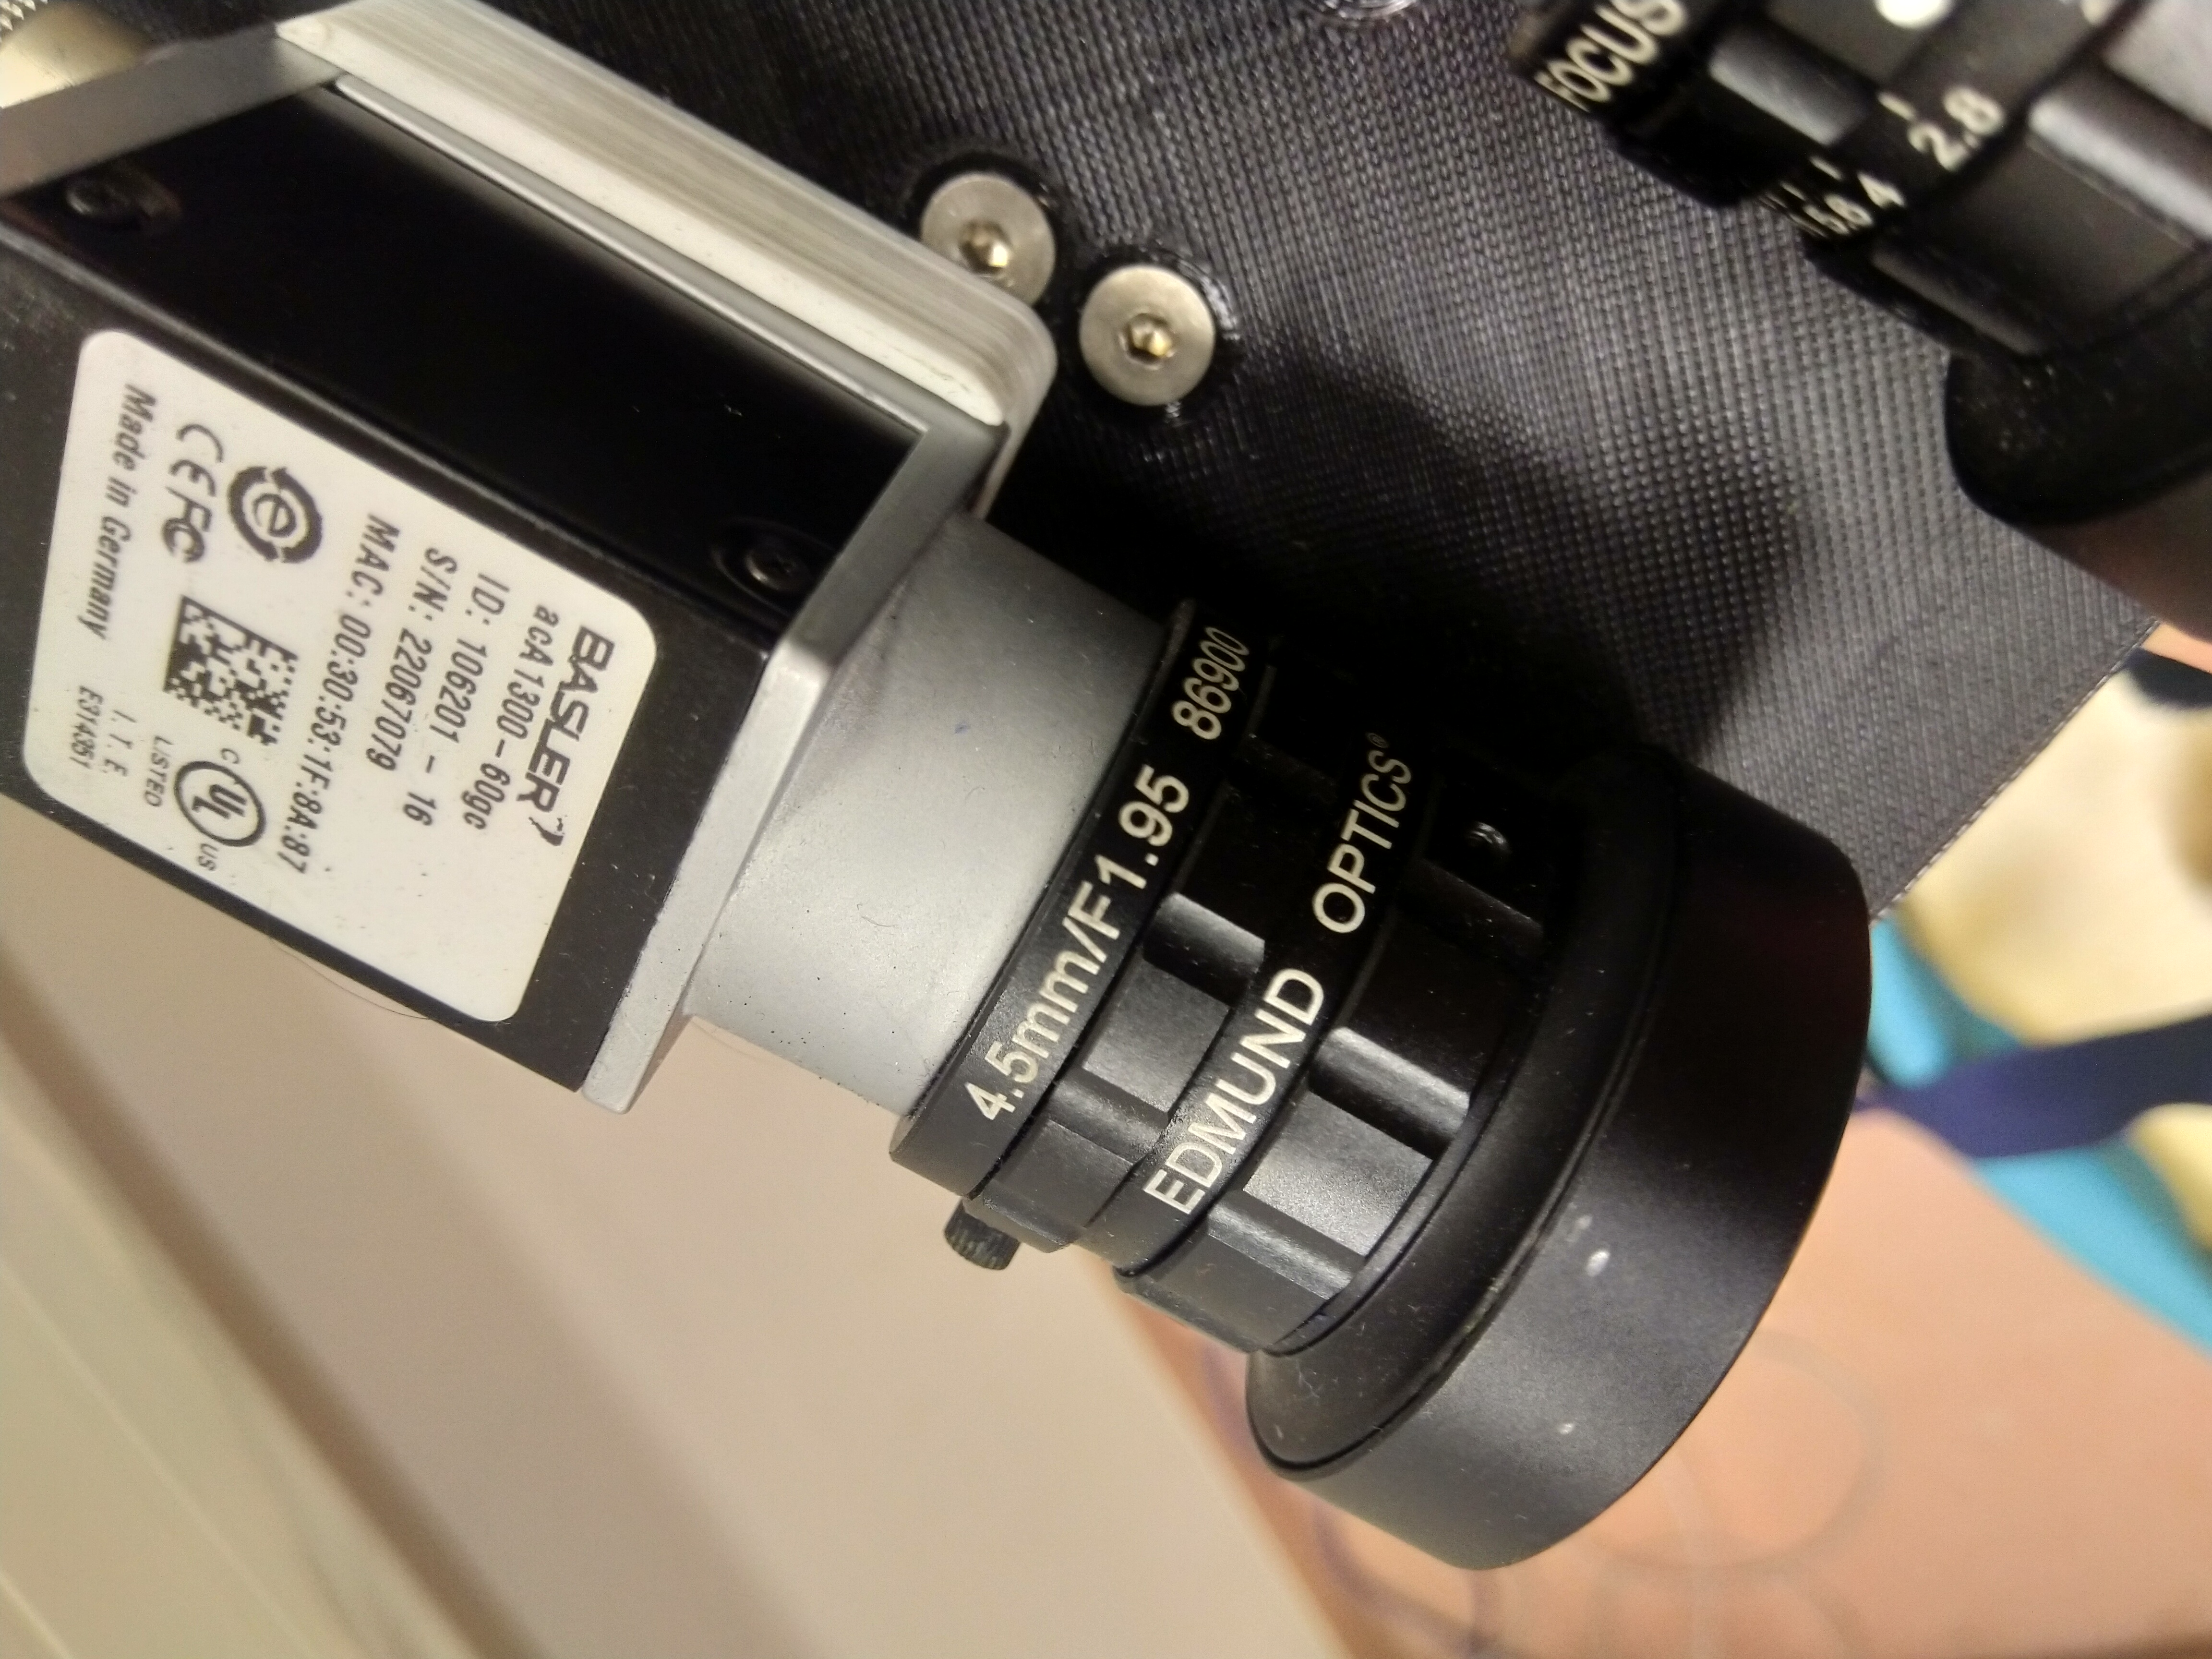
\includegraphics[width=80mm, angle=180, keepaspectratio]{03_images/kamera1.jpg}
    \caption{BASLER acA1300-60gc kamera.}
    \label{fig:cam}
\end{figure}

Ebben a fejezetben a paraméterek kapcsolatáról írok. Minél kevesebb időt szeretnénk feldolgozásra fordítani, annál erősebb hardver szükséges. Egyértelműen minél több erőforrást tudunk a feldolgozásra biztosítani, annál gyorsabb lesz a folyamat. Minél jobb minőséget (nagyobb felbontást) szeretnénk elérni, annál nagyobb a hardveres követelmény. A jobb minőség több információt jelent, amivel az algoritmusnak számolnia kell. Ebből kifolyólag több számítási kapacitásra van igény. A minőség (felbontás) és gyorsaság közötti kapcsolat már következik az előzőkből. Az erőforrásokban mindenképpen kompromisszumot kell kötnünk, ezért fontos, hogy megtaláljuk azt a minőséget, ami még megfelel az információ elérésére, de nem lassítja a folyamatot, oly módon hogy az információ elértéktelenedjen. Megállapítható, hogy ez egy szigorúan valós idejű rendszer, mivel az információ, ami jelen esetben az jelenti, hogy milyen arcokat ismert fel a robot, tehát kik azok a személyek akik a látóterében tartózkodnak, az idő elteltével elértéktelenedik. 